\section{Cluster Validity}
For supervised classification we have a variety of measures to evaluate how good our model is. such as accuracy, precision, recall, etc\dots


\coolquote{
   For cluster analysis, the analogous question is how to evaluate the ``goodness'' of the resulting clusters?
}{}

``Clusters are in the eye of the beholder'', but we still want to evaluate them to avoid finding patterns in noise, compare clustering algorithms, or to compare clusters or sets of clusters.

\section{Towards cluster validation}

\begin{enumerate}
   \item 
   Determining the \textbf{clustering tendency} of a set of data, i.e., distinguishing whether non-random structure actually exists in the data.
   \item Comparing the results of a cluster analysis to externally known results, e.g., to externally given class labels.
   \item Evaluating how well the results of a cluster analysis fit the data without reference to external information.
   \item Comparing the results of two different sets of cluster analyses to determine which is better
   \item Determining the ``correct'' number of clusters.
\end{enumerate}

Numerical measures that are applied to judge various aspects of cluster validity, are classified into the following three types:
\begin{itemize}
   \item \textbf{External} Index: Used to measure the extent to which cluster labels
match externally supplied class labels.
\note{Entropy}
\item \textbf{Internal} Index: Used to measure the goodness of a clustering
structure without respect to external information.
\note{Sum of Squared Error (SSE)}
\item \textbf{Relative} Index: Used to compare two different clusterings or
clusters.
\note{Often an external or internal index is used for this function, e.g., SSE or entropy}
\end{itemize}
Sometimes these are referred to as \textit{\textbf{criteria}} instead of \textit{indices}; however, sometimes criterion is the general strategy and index is the numerical measure that implements the criterion.

\subsection{Measuring validity through correlation}

Two matrices:
\begin{itemize}
   \item Proximity matrix
   \item Ideal similarity matrix
   \begin{itemize}
      \item One row and one column for each data point
      \item An entry is 1 if the associated pair of points belong to the same cluster
      \item An entry is 0 if the associated pair of points belongs to different clusters
   \end{itemize}
\end{itemize}

Compute the correlation between the two matrices; note that since the matrices are symmetric, only the correlation between $n(n-1) / 2$ entries needs to be calculated.

\begin{figure}[htbp]
   \centering
   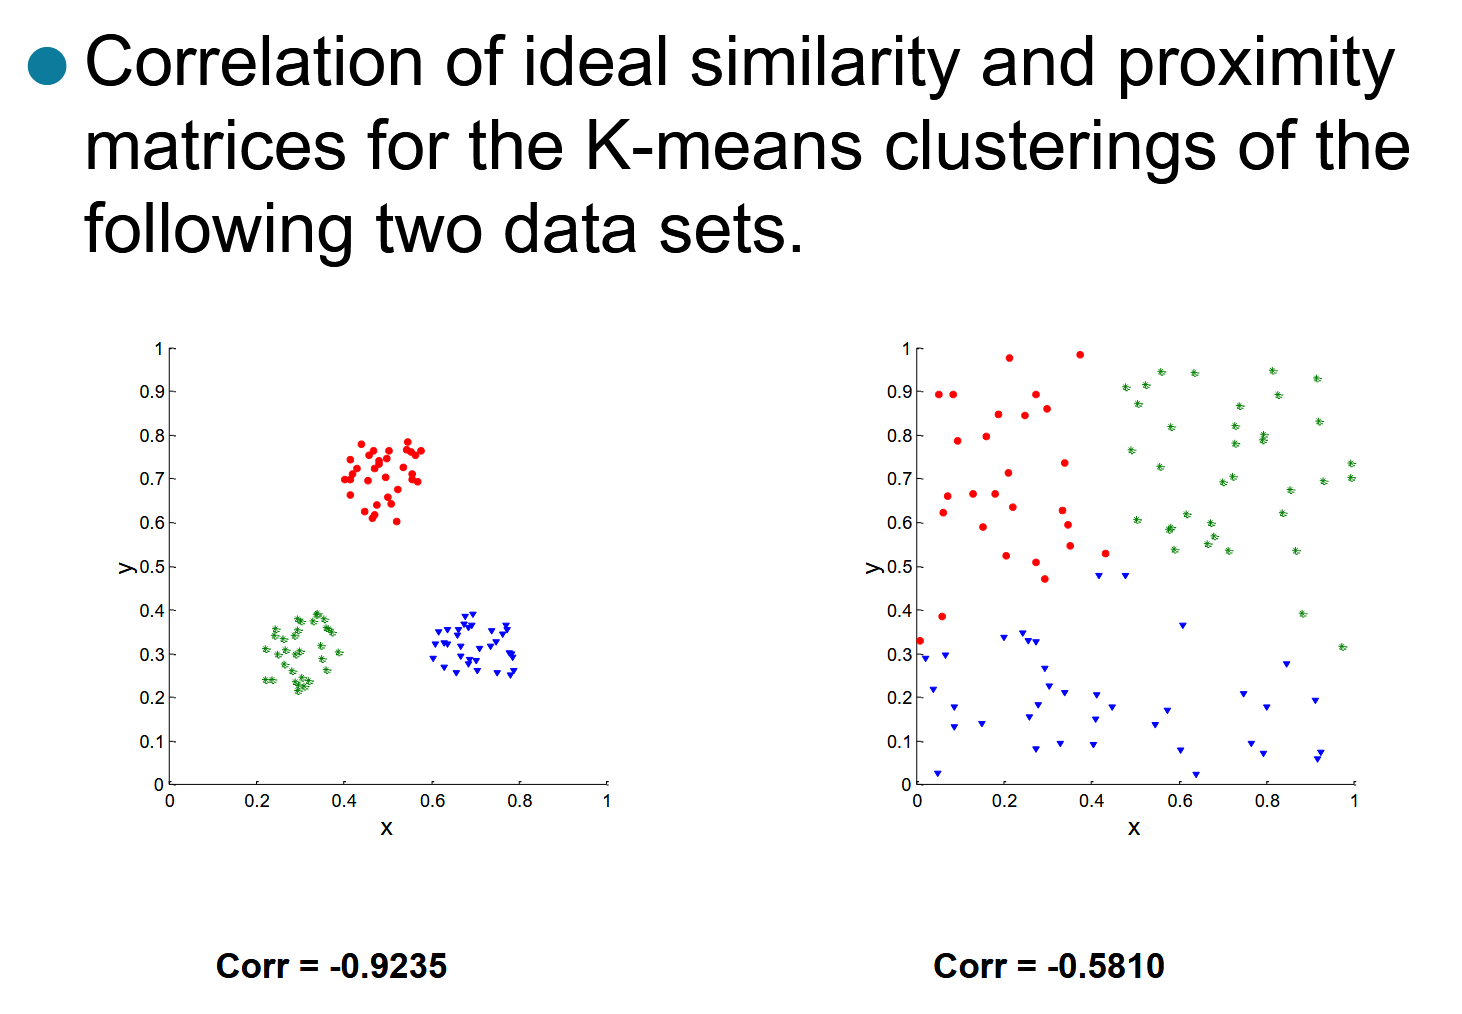
\includegraphics{images/05/correlation.png}
   \caption{Correlation of two sets. Actually, in real world data it's very rare to observe a $-0.9235$ correlation score}
   \label{fig:correlation}
\end{figure}

\subsection{Internal measures}


\subsubsection{SSE - Sum of Squared Error}
\begin{paracol}{2}
   
   
   \begin{figure}[htbp]
      \centering
      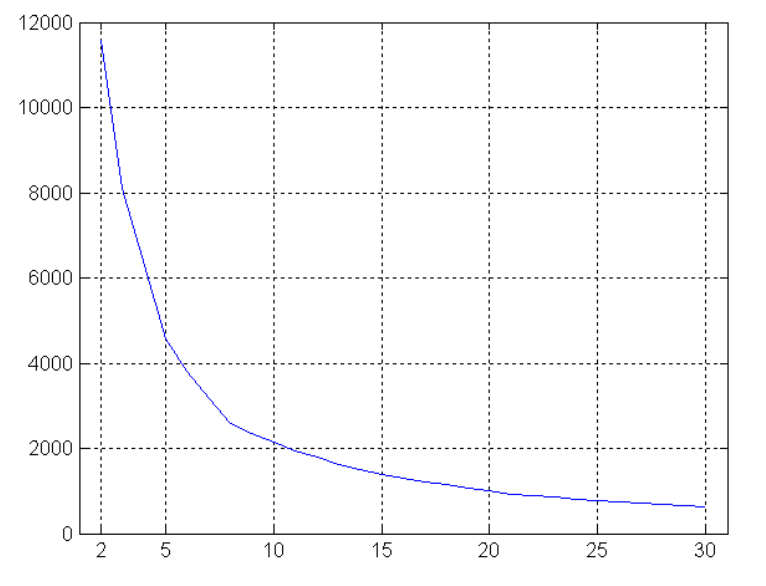
\includegraphics{images/05/sse.png}
      \caption{SSE of cluster found using K-means with various values of $k$}
      \label{fig:05/sse}
   \end{figure}
   
   \switchcolumn
   
   SSE (Sum of Squared Error) is a common measure of cluster cohesion, defined as:
   \[SSE = \sum_{i=1}^{k} \sum_{x \in C_i} dist^2(m_i, x)\]
   where $m_i$ is the centroid of cluster $C_i$.
   
   This is a measure of how tightly the data points in a cluster are grouped together. Lower values of SSE indicate more cohesive clusters.
   It can be a nice measure which does not need external information, and may also be used to determine the appropriate number of clusters by plotting the SSE for different values of $k$ and looking for an ``elbow'' in the graph.
\end{paracol}

\subsubsection{Cohesion and Separation}

\begin{figure}[htbp]
   \centering
   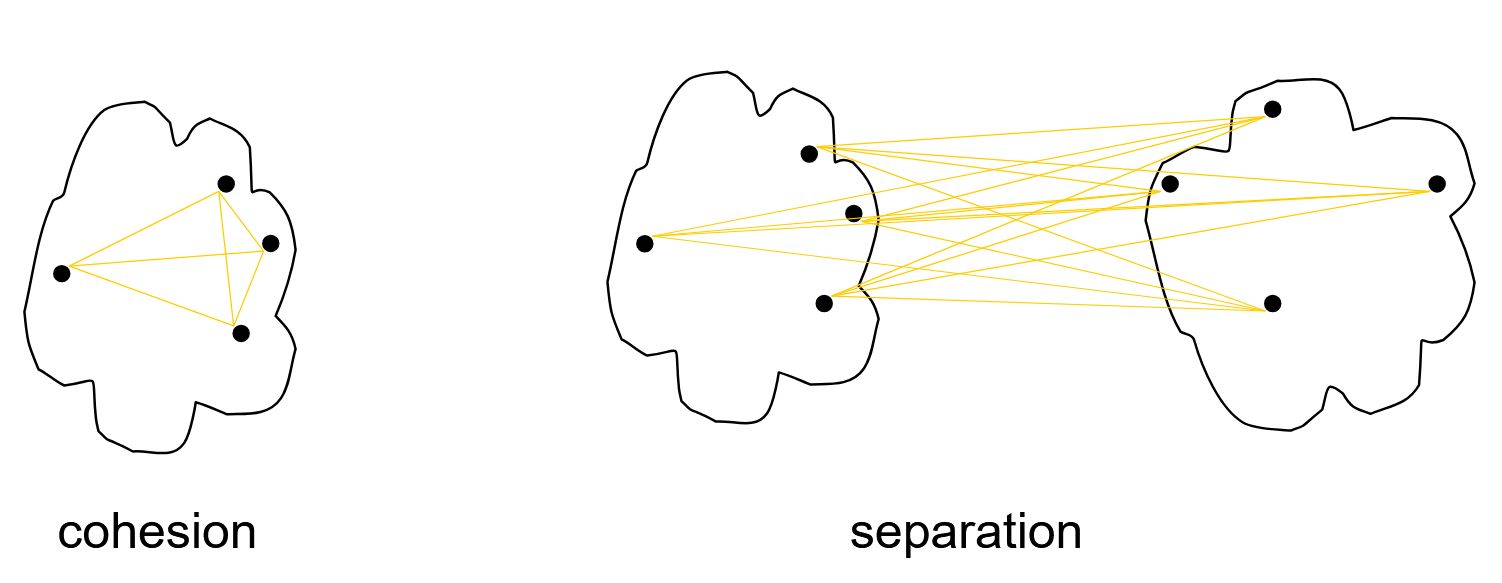
\includegraphics{images/05/cohesion.png}
   \caption{Cohesion and separation}
   \label{fig:05/cohesion}
\end{figure}
A proximity graph based approach can also be used for
cohesion and separation.
\begin{itemize}
	\item Cluster \textbf{cohesion} is the sum of the weight of all links within a cluster, it measures how closely related are objects in a cluster. (SSE is a measure of cohesion)
	\[
   SSE = WSS = \sum_i \sum_{x \in C_i}(x - m_i)^2
   \]
	\item Cluster \textbf{separation} is the sum of the weights between nodes in the cluster and nodes outside the cluster.
	Measures how distinct or well-separated a cluster is from other clusters. (Squared error between clusters is a measure of separation)
   \[
   BSS = \sum_i|C_i|(m-m_i)^2 \qquad |C_i| \text{ size of cluster } C_i
   \]

   Note that $BSS + WSS = TSS$ where $TSS$ is the total sum of squares, and is constant and independent of the clustering.
\end{itemize}

\subsubsection{Silhouette coefficient}
Silhouette coefficient combines ideas of both cohesion and separation,
but for individual points, as well as clusters and clusterings.
\begin{paracol}{2}

	Consider a point $i$ in cluster $A$:
	\begin{itemize}
		\item Calculate $a$ = average distance of $i$ to the points in its cluster
		\item Calculate $b$ = min (average distance of $i$ to points in another cluster)
		\item The silhouette coefficient for a point is then given by
		      \[
			      s = \frac{b - a}{\max(a,b)}
		      \]
		\item Typically between $0$ and $1$. The closer to $1$ the better.
		\item Can calculate the average silhouette coefficient for a cluster or a clustering.
	\end{itemize}
	\switchcolumn

   \colfill
	\begin{figure}[htbp]
		\centering
		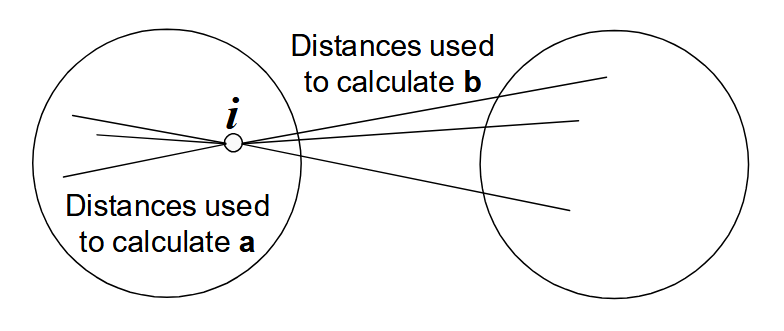
\includegraphics[width=0.95\columnwidth]{images/05/silhouette.png}
		\caption{Silhouette coefficient for $i$}
		\label{fig:05/silhouette}
	\end{figure}
   \colfill
\end{paracol}

\subsection{External measures}
External measures compare the clustering results to an externally known class labels. Examples may be \textbf{entropy} and \textbf{purity}.

\begin{table}[htbp]
\centering
\caption{K-means Clustering Results for LA Document Data Set}
\label{tab:05/kmeans_results}
\begin{tabular}{|c|c|c|c|c|c|c|c|c|}
\hline
\textbf{Cluster} & \textbf{Entertainment} & \textbf{Financial} & \textbf{Foreign} & \textbf{Metro} & \textbf{National} & \textbf{Sports} & \textbf{Entropy} & \textbf{Purity} \\
\hline
1 & 3 & 5 & 40 & 506 & 96 & 27 & 1.2270 & 0.7474 \\
\hline
2 & 4 & 7 & 280 & 29 & 39 & 2 & 1.1472 & 0.7756 \\
\hline
3 & 1 & 1 & 1 & 7 & 4 & 671 & 0.1813 & 0.9796 \\
\hline
4 & 10 & 162 & 3 & 119 & 73 & 2 & 1.7487 & 0.4390 \\
\hline
5 & 331 & 22 & 5 & 70 & 13 & 23 & 1.3976 & 0.7134 \\
\hline
6 & 5 & 358 & 12 & 212 & 48 & 13 & 1.5523 & 0.5525 \\
\hline
\textbf{Total} & 354 & 555 & 341 & 943 & 273 & 738 & 1.1450 & 0.7203 \\
\hline
\end{tabular}
\end{table}

\subsubsection{Entropy}
Entropy measures how the various clusters are distributed with respect to the class labels.

For each cluster, the class distribution of the data is calculated first, i.e., for cluster $j$ we compute $p_{ij}$, the ``probability'' that a member of cluster $j$ belongs to class $i$ as follows: $p_{ij} = m_{ij}/m_j$, where $m_j$ is the number of values in cluster $j$ and $m_{ij}$ is the number of values of class $i$ in cluster $j$. 

Then using this class distribution, the entropy of \textit{each} cluster $j$ is calculated using the standard formula:
\[
e_j = -\sum_{i=1}^{L} p_{ij} \log_2 p_{ij}
\]
where $L$ is the number of classes. 

The total entropy for a set of clusters is calculated as the sum of the entropies of each cluster weighted by the size of each cluster, i.e.:
\[
e = \sum_{i=1}^{K} \frac{m_i}{m} e_j
\]
where $m_j$ is the size of cluster $j$, $K$ is the number of clusters, and $m$ is the total number of data points.

\subsubsection{Purity}
Using the terminology derived for entropy, the purity of cluster $j$, is given by:
\[
purity_j = \max_i p_{ij}
\]
and the overall purity of a clustering by:
\[
purity = \sum_{i=1}^{K} \frac{m_i}{m} purity_j
\]



